\documentclass{beamer}


\usepackage{amssymb,amsmath}
\usepackage{graphicx}
\usepackage{url}
\usepackage{color}
\usepackage{relsize}		% For \smaller
\usepackage{url}			% For \url
\usepackage{epstopdf}	% Included EPS files automatically converted to PDF to include with pdflatex

%For MindMaps
% \usepackage{tikz}%
% \usetikzlibrary{mindmap,trees,arrows}%

%%% Color Definitions %%%%%%%%%%%%%%%%%%%%%%%%%%%%%%%%%%%%%%%%%%%%%%%%%%%%%%%%%
%\definecolor{bordercol}{RGB}{40,40,40}
%\definecolor{headercol1}{RGB}{186,215,230}
%\definecolor{headercol2}{RGB}{80,80,80}
%\definecolor{headerfontcol}{RGB}{0,0,0}
%\definecolor{boxcolor}{RGB}{186,215,230}

%%% Save space in lists. Use this after the opening of the list %%%%%%%%%%%%%%%%
%\newcommand{\compresslist}{
%	\setlength{\itemsep}{1pt}
%	\setlength{\parskip}{0pt}
%	\setlength{\parsep}{0pt}
%}

%\setbeameroption{show notes on top}

% You should run 'pdflatex' TWICE, because of TOC issues.

% Rename this file.  A common temptation for first-time slide makers
% is to name it something like ``my_talk.tex'' or
% ``john_doe_talk.tex'' or even ``discrete_math_seminar_talk.tex''.
% You really won't like any of these titles the second time you give a
% talk.  Try naming your tex file something more descriptive, like
% ``riemann_hypothesis_short_proof_talk.tex''.  Even better (in case
% you recycle 99% of a talk, but still want to change a little, and
% retain copies of each), how about
% ``riemann_hypothesis_short_proof_MIT-Colloquium.2000-01-01.tex''?

\mode<presentation>
{
  % A tip: pick a theme you like first, and THEN modify the color theme, and then add math content.
  % Warsaw is the theme selected by default in Beamer's installation sample files.

  %%%%%%%%%%%%%%%%%%%%%%%%%%%% THEME
  %\usetheme{AnnArbor}
  %\usetheme{Antibes}
  %\usetheme{Bergen}
  %\usetheme{Berkeley}		% bem bacana - menu esquerdo
  %\usetheme{Berlin}
  %\usetheme{Boadilla}
  %\usetheme{boxes}
  %\usetheme{CambridgeUS}		% bem bacana - menu superior
  %\usetheme{Copenhagen}
  %\usetheme{Darmstadt}
  %\usetheme{default}
  %\usetheme{Dresden}
  \usetheme{Frankfurt}
  %\usetheme{Goettingen}
  %\usetheme{Hannover}		% bem bacana - menu esquerdo
  %\usetheme{Ilmenau}
  %\usetheme{JuanLesPins}
  %\usetheme{Luebeck}
  %\usetheme{Madrid}		%bacana
  %\usetheme{Malmoe}
  %\usetheme{Marburg}		% bem bacana - menu direito
  %\usetheme{Montpellier}
  %\usetheme{PaloAlto}		% bem bacana - menu esquerdo
  %\usetheme{Pittsburgh}
  %\usetheme{Rochester}		%bacana
  %\usetheme{Singapore}
  %\usetheme{Szeged}
  %\usetheme{Warsaw}

  %%%%%%%%%%%%%%%%%%%%%%%%%%%% COLOR THEME
  %\usecolortheme{albatross}		% azul escuro, massa
  %\usecolortheme{beetle}		% cinza, menu azul
  %\usecolortheme{crane}		% branco e amarelo, massa
  \usecolortheme{default}		% branco, azul clarinho
  %\usecolortheme{dolphin}		% azul e branco, legal
  %\usecolortheme{dove}			% cinza e branco, feio
  %\usecolortheme{fly}			% todo cinza, horrível
  %\usecolortheme{lily}			% parece o default
  %\usecolortheme{orchid}		% azul e branco, ok
  %\usecolortheme{rose}			% branco e violeta-claro, bonito
  %\usecolortheme{seagull}		% cinza, feio
  %\usecolortheme{seahorse}		% nhé, meio feio
  %\usecolortheme{sidebartab}		% Azul, branco, destaque na tab, interessante
  %\usecolortheme{structure}		% bichado
  %\usecolortheme{whale}		% Azul e branco, bem bonito

  %%%%%%%%%%%%%%%%%%%%%%%%%%%% OUTER THEME
  \useoutertheme{default}
  %\useoutertheme{infolines}
  %\useoutertheme{miniframes}
  %\useoutertheme{shadow}
  %\useoutertheme{sidebar}
  %\useoutertheme{smoothbars}
  %\useoutertheme{smoothtree}
  %\useoutertheme{split}
  %\useoutertheme{tree}

  %%%%%%%%%%%%%%%%%%%%%%%%%%%% INNER THEME
  \useinnertheme{circles}
  %\useinnertheme{default}
  %\useinnertheme{inmargin}
  %\useinnertheme{rectangles}
  %\useinnertheme{rounded}

  %%%%%%%%%%%%%%%%%%%%%%%%%%%%%%%%%%%

  \setbeamercovered{invisible} % or whatever (possibly just delete it)
  % To change behavior of \uncover from graying out to totally
  % invisible, can change \setbeamercovered to invisible instead of
  % transparent. apparently there are also 'dynamic' modes that make
  % the amount of graying depend on how long it'll take until the
  % thing is uncovered.

}


% Get rid of nav bar
\beamertemplatenavigationsymbolsempty

% Use short top
%\usepackage[headheight=12pt,footheight=12pt]{beamerthemeboxes}
%\addheadboxtemplate{\color{black}}{
%\hskip0.5cm
%\color{white}
%\insertshortauthor \ \ \ \ 
%\insertframenumber \ \ \ \ \ \ \ 
%\insertsection \ \ \ \ \ \ \ \ \ \ \ \ \ \ \ \ \  \insertsubsection
%\hskip0.5cm}
%\addheadboxtemplate{\color{black}}{
%\color{white}
%\ \ \ \ 
%\insertsection
%}
%\addheadboxtemplate{\color{black}}{
%\color{white}
%\ \ \ \ 
%\insertsubsection
%}

% Insert frame number at bottom of the page.
% \usefoottemplate{\hfil\tiny{\color{black!90}\insertframenumber}} 

\usepackage[english]{babel}
\usepackage[latin1]{inputenc}
\usepackage{subfigure}

\usepackage{times}
\usepackage[T1]{fontenc}


\title[GB21802]{GB21802 - Programming Challenges}
\subtitle[]{Week 0 - Introduction}
\author[Claus Aranha]{Claus Aranha\\{\footnotesize caranha\@@cs.tsukuba.ac.jp}}
\institute{Department of Computer Science}
\date{2019/4/12\\{\smaller(last updated: \today)}}

\begin{document}

\section{Introduction}
\begin{frame}
\maketitle
\end{frame}

\subsection{Crash Course}
\begin{frame}
  \frametitle{What is a Programming Challenge? - 0}

  Consider a string with $N$ characters chosen from $G,C,T,A$. Ex:

  \begin{center}
    \emph{\alert<2>{GACA\alert<4>{CATACAG}AT}TA\alert<3>{CATTAC}AGA ... GATACCAGATA}
  \end{center}

  When you receive pair of indexes $s$ and $e$, calculate the number of "CA"s between $N_s$ and $N_e$. Ex:

  \begin{itemize}
    \item \only<2->{s = 0, e = 12\hfill 3 repetitions}
    \item \only<3->{s = 15, e = 20\hfill 1 repetition}
    \item \only<4>{s = 4, e = 10\hfill 2 repetitions}
  \end{itemize}
\end{frame}

\begin{frame}[t]
  \frametitle{What is a Programming Challenge? - 1}

  \begin{center}
    \emph{GACACATACAGATTACATTACAGA ... GATACCAGATA}
    \only<2>{\emph{000112222333333344444555 ... 88888899999}}
  \end{center}

  \begin{block}{Algorithm Idea 1}
    Start a counter $c = 0$, loop from $N_s$ to $N_e$,
    and every time you find "CA", add to the counter.
    \bigskip

    \alert{Problem: If we have many queries, can we do faster?}
  \end{block}

  \begin{onlyenv}<2>

  \begin{block}{Algorithm Idea 2}
    Creat an auxiliary array $A$, that keeps the \alert{Cummulative sum} of "CA"s from $N_0$ to $N_i$.

    \bigskip

    If we want to know the answer, we calculate $A_e - A_s$.
  \end{block}
  \end{onlyenv}
\end{frame}


\begin{frame}
  \frametitle{What is a Programming Challenge? - 2}

  \begin{itemize}
    \item Program Challenges are good for \structure{Practicing Algorithms}
    \bigskip

    \item Program Challenges are good for \structure{Rapid Prototyping}
    \bigskip

    \item Program Challenges are used for \structure{Work Recruiting}
    \bigskip

    \item Program Challenges are also \structure{very fun puzzles!}
  \end{itemize}
\end{frame}

\begin{frame}
  \frametitle{This course is about Programming Challenges}

  The Goal of this course is \structure{solve programming challenges} to \alert{become better at programming}.

  \vfill

  We will study \structure{algorithms and techniques} that are common in
  \structure{programming competitions}
\end{frame}

\subsection{Course Outline}
\begin{frame}
  \frametitle{First Things First: Important Notices}

  \begin{block}{Manaba Page}
    All lecture notes and announcements for this course will be done
    through MANABA. Access the url below:

    \medskip

    \url{https://manaba.tsukuba.ac.jp/ct/course_1149028}\\
    Registration Code: 7255921
  \end{block}
  \begin{exampleblock}{Language}
    \begin{itemize}
      \item \structure{Lectures}: Japanese
      \item \structure{Slides and materials}: English
      \item \structure{Exercises}: English
      \item \structure{Questions, Mails and Homework}: Any language
    \end{itemize}
  \end{exampleblock}
\end{frame}

\begin{frame}
  \frametitle{About the Lecturer}
  \begin{columns}
    \column{0.4\textwidth}
    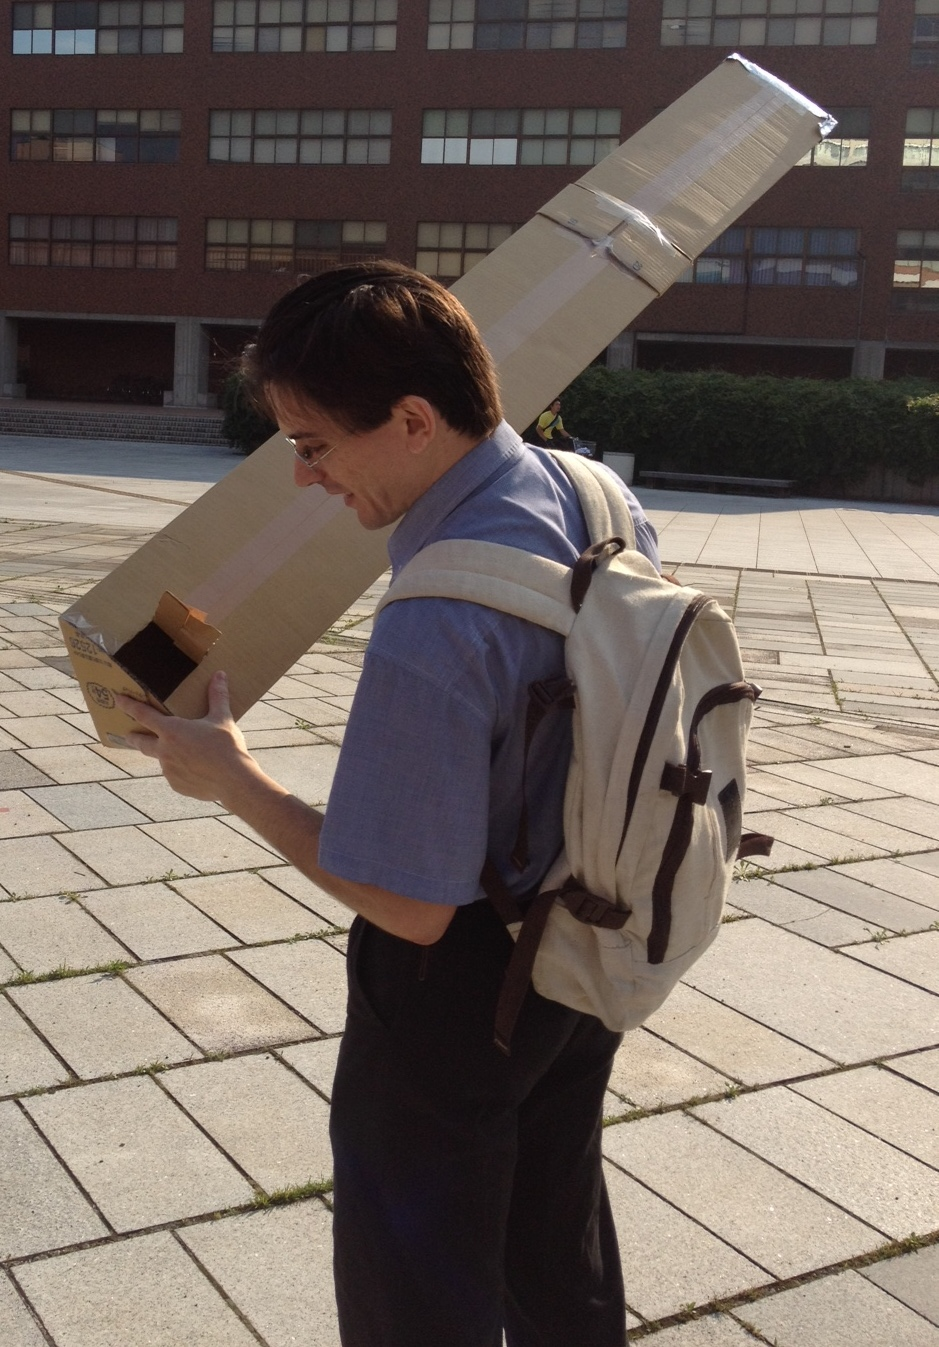
\includegraphics[width=1\textwidth]{../img/pinhole}
    \column{0.6\textwidth}
    {\small
    \begin{itemize}
      \item \structure{Name:} Claus Aranha;
      \item \structure{Country:} Brazil;

        \medskip

      \item \structure{Research:} Artificial Intelligence,
        Evolutionary Algorithms, Genetic Programming;
      \item \structure{Language:} Python, R;
      \item \structure{Hobbies:} Game Programming, Geocaching;

        \medskip

      \item \structure{webpage:}\\ {\smaller \url{http://conclave.cs.tsukuba.ac.jp}}
    \end{itemize}
    }
  \end{columns}
\end{frame}

\begin{frame}
  \frametitle{What is this course about?}

  You have learned many programming techniques...\\\hfill \structure{...but can you use them?}

  \begin{block}{Course Objective: Learning by Practice}
    \begin{itemize}
      {\small
    \item Every week: Solve 8 programming challenges;
    \item \structure{Choose} and \structure{implement} the {\bf best algorithm} for each problem;
    \item Be careful with \alert{max time}, and \alert{max memory};
    \item We will discuss algorithms, techniques and tricks;
      }
    \end{itemize}
  \end{block}

  \begin{exampleblock}{Course Goal:}
    Improve programming abilities, techniques and familiarity.
  \end{exampleblock}
\end{frame}

\begin{frame}
  \frametitle{Warnings about this class}
  \begin{alertblock}{1- Heavy Workload}
    \begin{itemize}
    \item Starts easy, but hard in the end;
    \item A few hours/week of homework;
    \item Lots of debugging;

      \bigskip

    \item Hint: Do your homework early!
    \end{itemize}
  \end{alertblock}

  \begin{alertblock}{2- Course Language}
    \begin{itemize}
    \item My Japanese is not very good ;-) Let's talk in C++!
    \item All the course materials are in English;
    \item You can make your homework in Japanese;

      \bigskip

    \item Practice some English in this course too! :-)
    \end{itemize}
  \end{alertblock}

\end{frame}

\section{Programming Challenges}
\subsection{Example}

\begin{frame}
  \frametitle{What is a ``Programming Challenge''?}

  A \structure{puzzle} that you solve by \structure{programming}.

  \bigskip

  Parts of a Programming Challenge:
  \begin{itemize}
  \item Description;
  \item Standard input;
  \item Standard output;
  \item Examples;
  \end{itemize}

  \bigskip

  Task: Write a program that:
  \begin{itemize}
    \item Reads the input;
    \item Prints the \structure{correct} output;
    \item And nothing else!
  \end{itemize}
\end{frame}

\subsection{Tutorial}
\begin{frame}
  \frametitle{Tutorial: ``Relational Operator'' (1)}

  All challenges are listed at the page:\\
  {\smaller \url{http://conclave.cs.tsukuba.ac.jp/lecture/monitor.html}}

  \bigskip

  Let's click on "Relational Operator"

  \begin{center}
    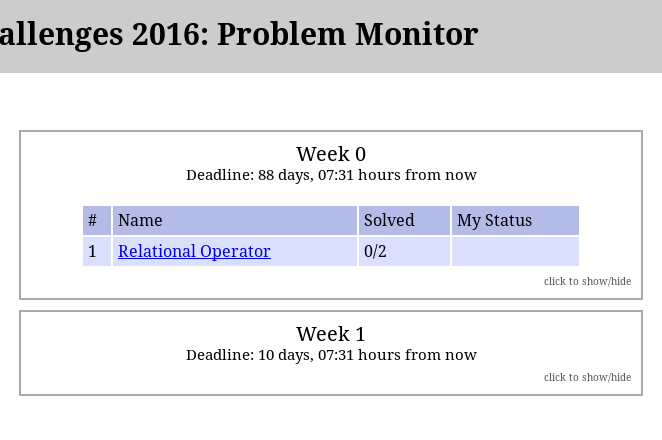
\includegraphics[width=.7\textwidth]{../img/monitorpage}
  \end{center}

\end{frame}

\begin{frame}
  \frametitle{Tutorial: ``Relational Operator'' (2)}

  The link takes you to the UVA (University of Valladolid) homepage (\alert{Please use an ad blocker!}).

  \bigskip

  Here you can see the problem description, and the links to submit the problem.

  \begin{center}
    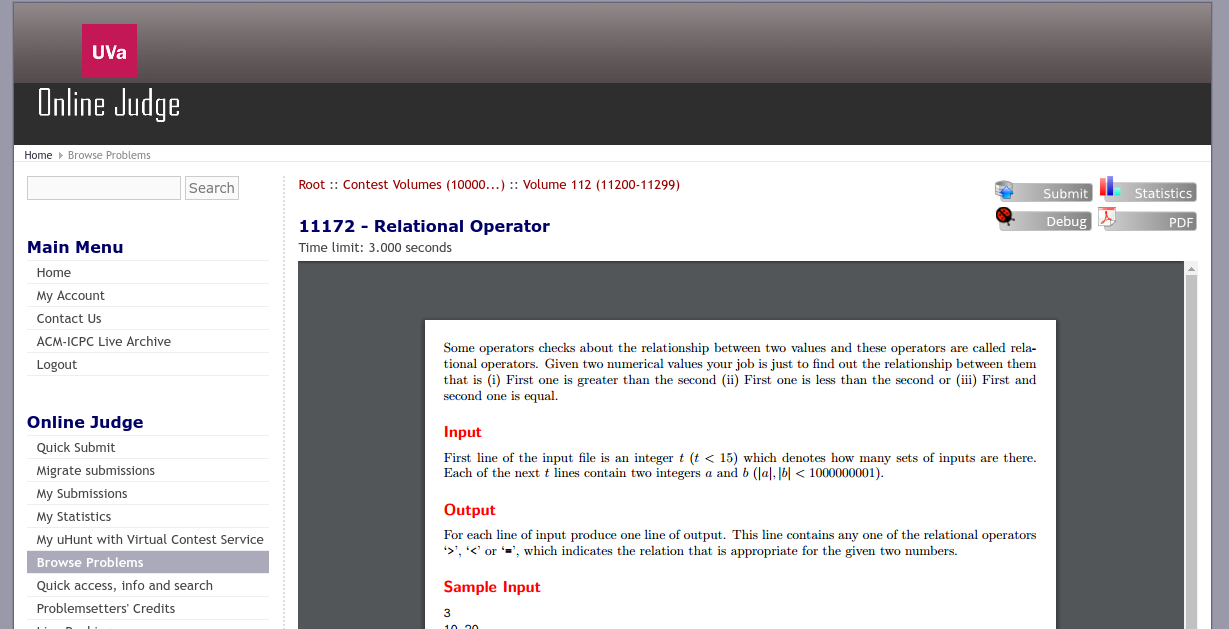
\includegraphics[width=.9\textwidth]{../img/relationaloperator}
  \end{center}
\end{frame}

\begin{frame}
  \frametitle{Tutorial: ``Relational Operator'' (3)}

  \begin{block}{Description}
    {\smaller \emph{
    Some operators checks about the relationship between two values and these
    operators are called relational operators. Given two numerical values \alert{your
    job is} just to find out the relationship between them that is (i) First one
    is greater than the second (ii) First one is less than the second or (iii)
    First and second one is equal.}}
  \end{block}

  \begin{itemize}
    \item Reading the description can be the hardest part!
    \item For this challenge, you just need to:
    \begin{itemize}
      \item If the first number is bigger than the second; print ">"
      \item If the first number is smaller than the second; print "<"
      \item If both numbers are equal, print "="
    \end{itemize}
  \end{itemize}
  Very easy!
\end{frame}


\begin{frame}
  \frametitle{Tutorial: ``Relational Operator'' (4)}

  \begin{block}{Input and Output}
    {\smaller
    \alert{Input}\\
    First line of the input file is an integer $t (t < 15)$ which denotes how many sets of inputs are there.
    Each of the next t lines contain two integers a and b (|a|, $|b| < 1000000001$).
    \medskip

    \alert{Output}\\
    For each line of input produce one line of output. This line  contains any one of the relational operators
    ''>'', ''<'' or ''='', which indicates the relation that is appropriate for the given two numbers.
  }
  \end{block}

  \begin{itemize}
    \item It is important to read the \alert{size} of the problem!
    \item Pay attention to the \alert{shape} of the output!
  \end{itemize}

\end{frame}

\begin{frame}
  \frametitle{Tutorial: ``Relational Operator'' (5)}
  \begin{block}{Examples}
  \alert{Sample Input}\\
  3\\
  10 20\\
  20 10\\
  10 10\\
  \alert{Sample Output}\\
  <\\
  >\\
  =\\
  \end{block}

  \begin{itemize}
    \item Use the samples to test/debug your program.
    \item Use your own samples too!
    \item Use the samples to \structure{understand} the challenge.
  \end{itemize}
\end{frame}



\begin{frame}[fragile]
  \frametitle{Solution: C++}

\begin{block}{}
{\smaller
\begin{verbatim}
// UVA 11172 - Relational Operator
// Test if a is bigger, smaller or equal to b

#include <iostream>
using namespace std;

int main()
{
    int n; long a, b;

    cin >> n;
    for (; n > 0; n--)
    {
        cin >> a >> b;
        if (a > b) cout << ">\n";
        if (a < b) cout << "<\n";
        if (a == b) cout << "=\n";
    }
}
\end{verbatim}}
\end{block}
\end{frame}

\begin{frame}[fragile]
  \frametitle{Solution: Python}
  \begin{block}{}
\begin{verbatim}
n = int(input())

while (n > 0):
   line = input()
   tokens = line.split()
   a,b = int(tokens[0]),int(tokens[1])

   if a > b: print(">")
   if a < b: print("<")
   if a == b: print("=")

   n -= 1
\end{verbatim}
  \end{block}

\end{frame}

\begin{frame}[fragile]
  \frametitle{Solution: Java}

  {\tiny
  \begin{block}{}
\begin{verbatim}
import java.io.*;
class Main
{
   public static void main(String args[])
   {
      BufferedReader stdin = new BufferedReader(new InputStreamReader(System.in));
      BufferedWriter stdout = new BufferedWriter(new OutputStreamWriter(System.out));
      try {
      String line;
      line = stdin.readLine();
      int n = Integer.parseInt(line);

      for (int i = 0; i < n; i++)
      {
         line = stdin.readLine();
         String[] tokens = line.split("\\s+");
         long a = Integer.parseInt(tokens[0]);
         long b = Integer.parseInt(tokens[1]);

         if (a > b)
            stdout.write(">\n");
         if (a < b)
            stdout.write("<\n");
         if (a == b)
            stdout.write("=\n");
         stdout.flush();
      }
      stdout.close();
      } catch (IOException ioe) { System.out.println("I/O Exception");}
   }
}
\end{verbatim}
  \end{block}
  }
\end{frame}

\begin{frame}
  \frametitle{Java Solution -- Keep in Mind}

  \begin{itemize}
  \item All code must be in the one file;

    \medskip

  \item The \structure{static main} method must be in \structure{Main} class.

    \medskip

  \item Do not use public classes. Even Main must be non public.

    \medskip

  \item Use Buffered I/O for faster input/output.
  \end{itemize}
\end{frame}

\subsection{Submitting Your Program}

\begin{frame}
  \frametitle{Submitting the problem to UVA}
  \begin{center}
    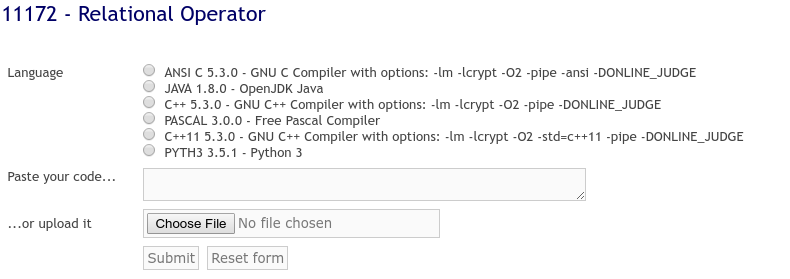
\includegraphics[width=1.1\textwidth]{../img/submitpage}
  \end{center}

  \begin{itemize}
    \item After you complete the program, use the \structure{submit} button in the UVA page;
    \item Choose your language and submit your code;
    \item You can choose C, C++, Java or Python.
  \end{itemize}
\end{frame}

\begin{frame}
  \frametitle{Submitting the problem to UVA}

    \begin{center}
      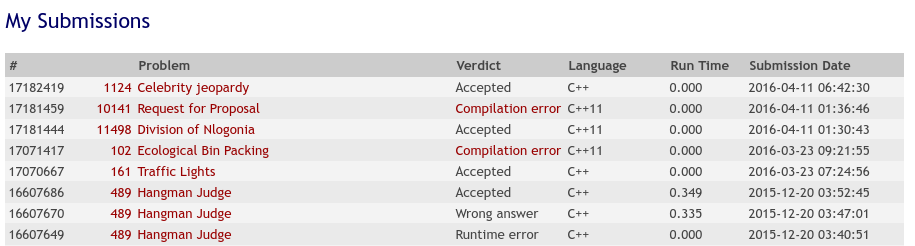
\includegraphics[width=1.1\textwidth]{../img/submissionpage}
    \end{center}

    \begin{itemize}
      \item UVA has an \structure{Automated Judge}.
      \item After 2~5 minutes, you should receive an e-mail with the result.
      \item All your results can be seen at "My Submissions" Page.
    \end{itemize}
\end{frame}

\begin{frame}
  \frametitle{Submitting the problem to UVA}

  These are the possible results:

  \bigskip

  \begin{itemize}
  \item \structure{Accepted}: Your program is correct!
    Congratulations!
  \item \structure{Presentation Error}: Small mistake in number of spaces. Congratulations!

    \bigskip

  \item \alert{Wrong Answer}: Your program is incorrect. Time to debug.

    \bigskip

  \item \alert{Time Limit Exceeded}: Your program is too slow.

  \item \alert{Memory limit exceeded}: Your program uses too much memory.

    \bigskip
  \item \alert{Runtime Error}: Your program crashed (segmentation fault!)

    \bigskip
  \end{itemize}

\end{frame}

\begin{frame}
  \frametitle{Problem Monitor Page}


  \begin{center}
    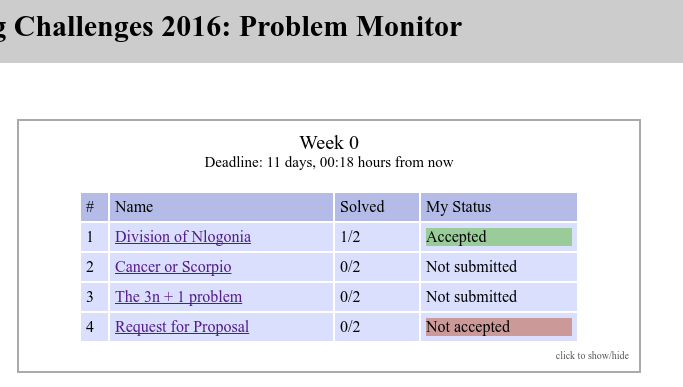
\includegraphics[width=1\textwidth]{../img/monitorpage2}
  \end{center}

  \begin{itemize}
    \item All Problems and results;
    \item All Deadlines;
  \end{itemize}

\end{frame}

\subsection{Manaba Submission}
\begin{frame}
  \frametitle{Submitting the problem to MANABA}

  {\small
  After you finish the problems listed in the monitor, you need to
  submit your source code and a comment file as a zip package to MANABA.}

  \medskip

  {\small
  \begin{columns}
    \column{0.3\textwidth}
    \column{0.4\textwidth}
    \begin{block}{s2015XXXXXX-weekYY.zip}
      \begin{itemize}
      \item problem1.cpp
      \item problem2.cpp
      \item problem5.cpp
      \item kaisetsu.txt
      \end{itemize}
    \end{block}
    \column{0.3\textwidth}
  \end{columns}
  }

  \medskip

  \begin{alertblock}{Attention}
  Submission to the UVA judge without a submission to MANABA will not
  be accepted!
  \end{alertblock}
\end{frame}

\section{Course Rules}
\subsection{Course Structure}

\begin{frame}
    \frametitle{Course Rules}

    \begin{block}{Two classes per week}
        \begin{itemize}
        \item Each week has a theme (Graphs, Maths, etc...)
        \item Friday Class: Introduction
        \item Monday Class: Problem Solving and Q\&A
        \end{itemize}
    \end{block}

    \begin{block}{Solving Problems}
        \begin{itemize}
        \item Every week there are 8 programming assignments;
        \item Deadline is Thursday 23:59
        \begin{itemize}
          \item UVA Submission
          \item MANABA Submission
        \end{itemize}
        \end{itemize}
    \end{block}
\end{frame}

\begin{frame}
  \frametitle{Outline}
  \begin{center}
    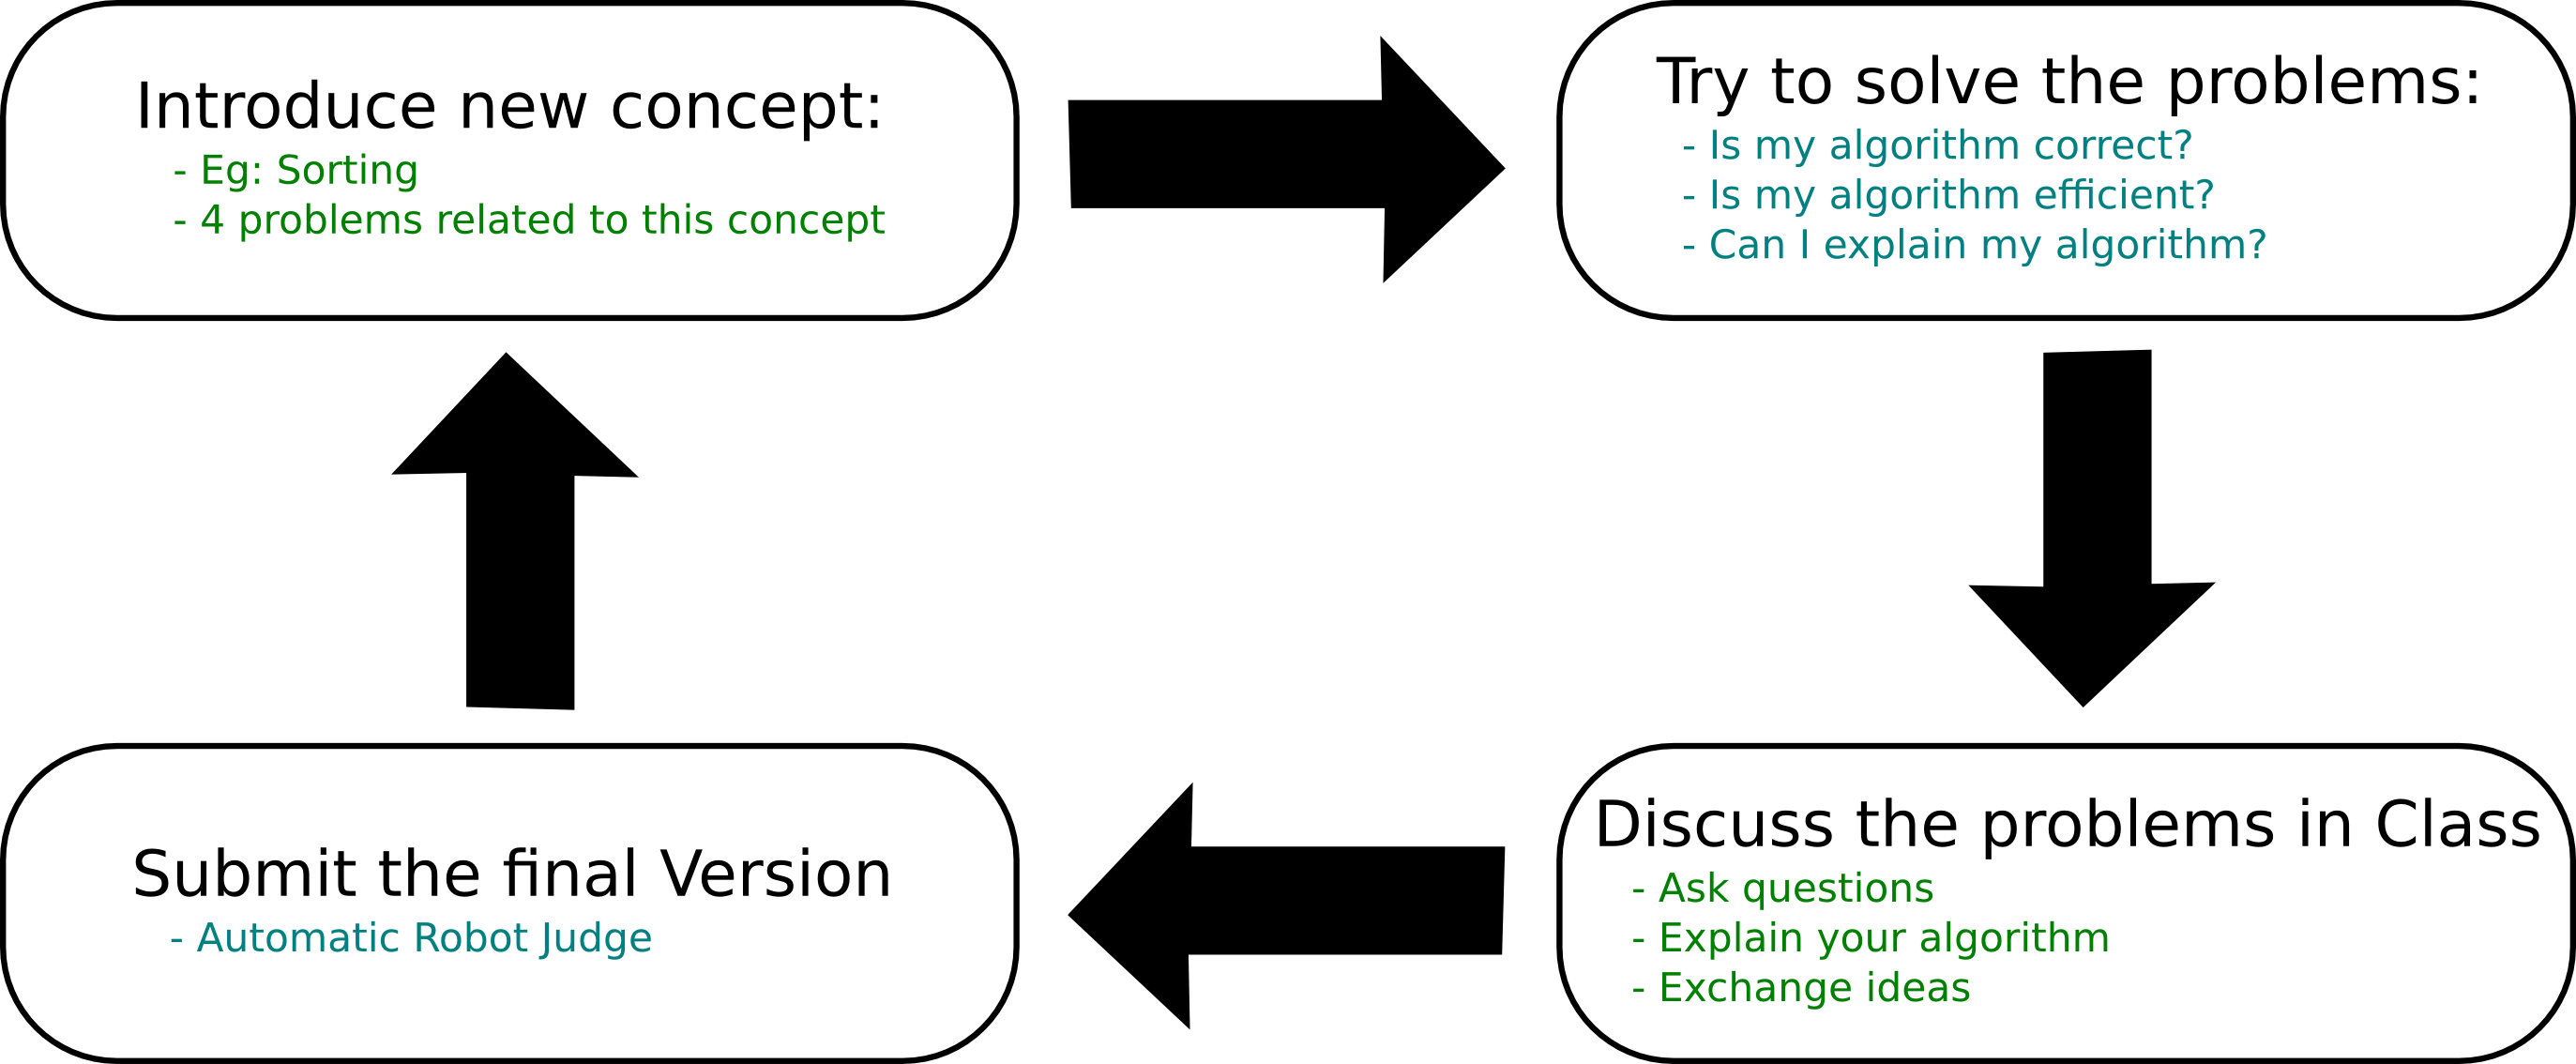
\includegraphics[width=1\textwidth]{../img/classoutline}
  \end{center}
\end{frame}

\subsection{Grading}

\begin{frame}
  \frametitle{Grading Algorithm}

  Your Grade: {\bf Base Grade} \structure{+Bonus} \alert{-Penalty}

  \begin{itemize}
    \item {\bf Base Grade}:
    \begin{itemize}
      \item You solved 2/8 problem/week: "C"
      \item You solved 3/8 problems/week: "B"
      \item You solved 4/8 problems/week: "A"
    \end{itemize}

    \bigskip

    \item \structure{+Bonus}
    \begin{itemize}
      \item 5\% of best student in each category.
      \item Special collaboration to the class.
    \end{itemize}

    \bigskip
    \item \alert{-Penalty}
    \begin{itemize}
      \item More than 25\% of homework submitted late.
    \end{itemize}
  \end{itemize}


\end{frame}

\begin{frame}[fragile]
  \frametitle{Evaluating and Grading: KAISETSU file}

  \begin{itemize}
    \item Submit a TEXT (not word) file with your impressions of the problems, class, life, together with your code.
    \item Kaisetsu file can be in any Japanese or English.
  \end{itemize}

  \bigskip

  \begin{exampleblock}{Example}
    {\smaller
\begin{verbatim}
Name: Claus, ID: 98884735
# Problem 1:
This problem was very easy, but I did a stupid mistake
and it took me three hours to solve. I found the solution
when I tried a new test case.

# Problem 2:
This problem was very hard, and I was very hungry, so I
gave up.
\end{verbatim}}
  \end{exampleblock}

\end{frame}

\begin{frame}
  \frametitle{Evaluation and Grading (5) -- about plagiarism}

  The assignments are \alert{individual}. Use your \structure{own
    strength} to solve the programs.

  \begin{exampleblock}{GOOD}
    \begin{itemize}
    \item Ask for ideas to your friends;
    \item Ask for ideas in the MANABA forum;
    \item Ask for help with a bug;
    \end{itemize}
  \end{exampleblock}

  \begin{alertblock}{BAD}
    \begin{itemize}
    \item Copy a solution from the internet;
    \item Copy a solution from your friends;
    \item Give your code to a friend;
    \end{itemize}
  \end{alertblock}

  Plagiarism will result in course failure, and possibly worse.
\end{frame}

\section{Resources}
\subsection{Resources}

% Class Links
\begin{frame}
  \frametitle{Useful Links}
  \begin{itemize}
  \item
    \href{https://manaba.tsukuba.ac.jp/ct/course_1149028}
         {\structure{\underline{Manaba Page}}}: All the class material
         will be here. Access Code is: 7255921

    \medskip

  \item \href{https://uva.onlinejudge.org/}{\structure{\underline{UVA Online Judge}}}:
    Use this page to submit your problems. \alert{Make an account and list the username on MANABA}

    \medskip

  \item \href{https://conclave.cs.tsukuba.ac.jp/lecture/monitor.html}{\structure{\underline{Problem Monitor}}}:
    Use this page to check deadlines and weekly problems.

    \medskip

  \item
    \href{https://www.github.com/caranha/ProgrammingChallengesLectureNotes}{\structure{\underline{Github
          Repository}}}:
    Working directory for lecture notes. Send me PR, issues!

    \medskip

  \item
    \href{https://www.udebug.com/}{\structure{\underline{uDebug}}}:
    Web service that generates test inputs and test outputs for UVA
    problems. Useful tool for this course.
  \end{itemize}
\end{frame}


% Books
% TODO: Add japanese books % Needs CJK package (or book images)
\begin{frame}
  \frametitle{Course Book}

  \begin{itemize}
  \item Competitive Programming, 3rd Edition
    (\href{http://cpbook.net/}{http://cpbook.net})

    \bigskip

  \item For suggestions of books in Japanese, please check the Manaba materials!
  \end{itemize}
\end{frame}

% udebug
\begin{frame}
  \frametitle{uDebug Tool}

  uDebug generates outputs for many different debugs. It can help you check why your program is wrong.

  \bigskip

  \url{https://www.udebug.com/}

  \bigskip

  \begin{center}
    
\includegraphics[width=0.7\textwidth]{../img/udebug}
  \end{center}
\end{frame}

% % Cat stream
% \begin{frame}
%   \frametitle{If you are still having problems...}
%
%   Watch a cat stream to relax!
%
%   \bigskip
%
%   \begin{center}
%     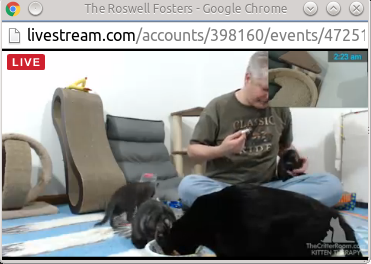
\includegraphics[width=.6\textwidth]{../img/catstream}
%   \end{center}
%
%   \bigskip
%
%   \url{http://livestream.com/FosterKittenCam/}
% \end{frame}


% Contact the professor (e-mail, twitter, webpage, room)
\begin{frame}
  \frametitle{Contact the professor}
  \begin{itemize}
  \item \structure{e-mail}: caranha@cs.tsukuba.ac.jp
  \item \structure{website}: \url{http://conclave.cs.tsukuba.ac.jp}
  %\item \structure{twitter}: @caranha

    \bigskip

  \item \structure{Room}: SB1012 -- Send an e-mail and we can talk!\\
  \end{itemize}

  \bigskip

  Both English and Japanese are okay!
\end{frame}


% Do we still have time? Fill out the forms!
% Do we still have time? Ask me questions!

\begin{frame}
  \frametitle{What to do this weekend?}

  \begin{itemize}
  \item Create an account on UVA (if you already have an account, you can use that)

    \bigskip

  \item Submit your account name to the MANABA

    \bigskip

  \item Ask any other questions you want to know!
  \end{itemize}
\end{frame}

\begin{frame}
  \frametitle{Participate in ICPC!}
  \begin{columns}
    \column{0.5\textwidth}
  \begin{itemize}
    \item Fun challenges to choose the world champion!
    \item Teams of 3 people!
    \item Registration Deadline Early of June!
  \end{itemize}

  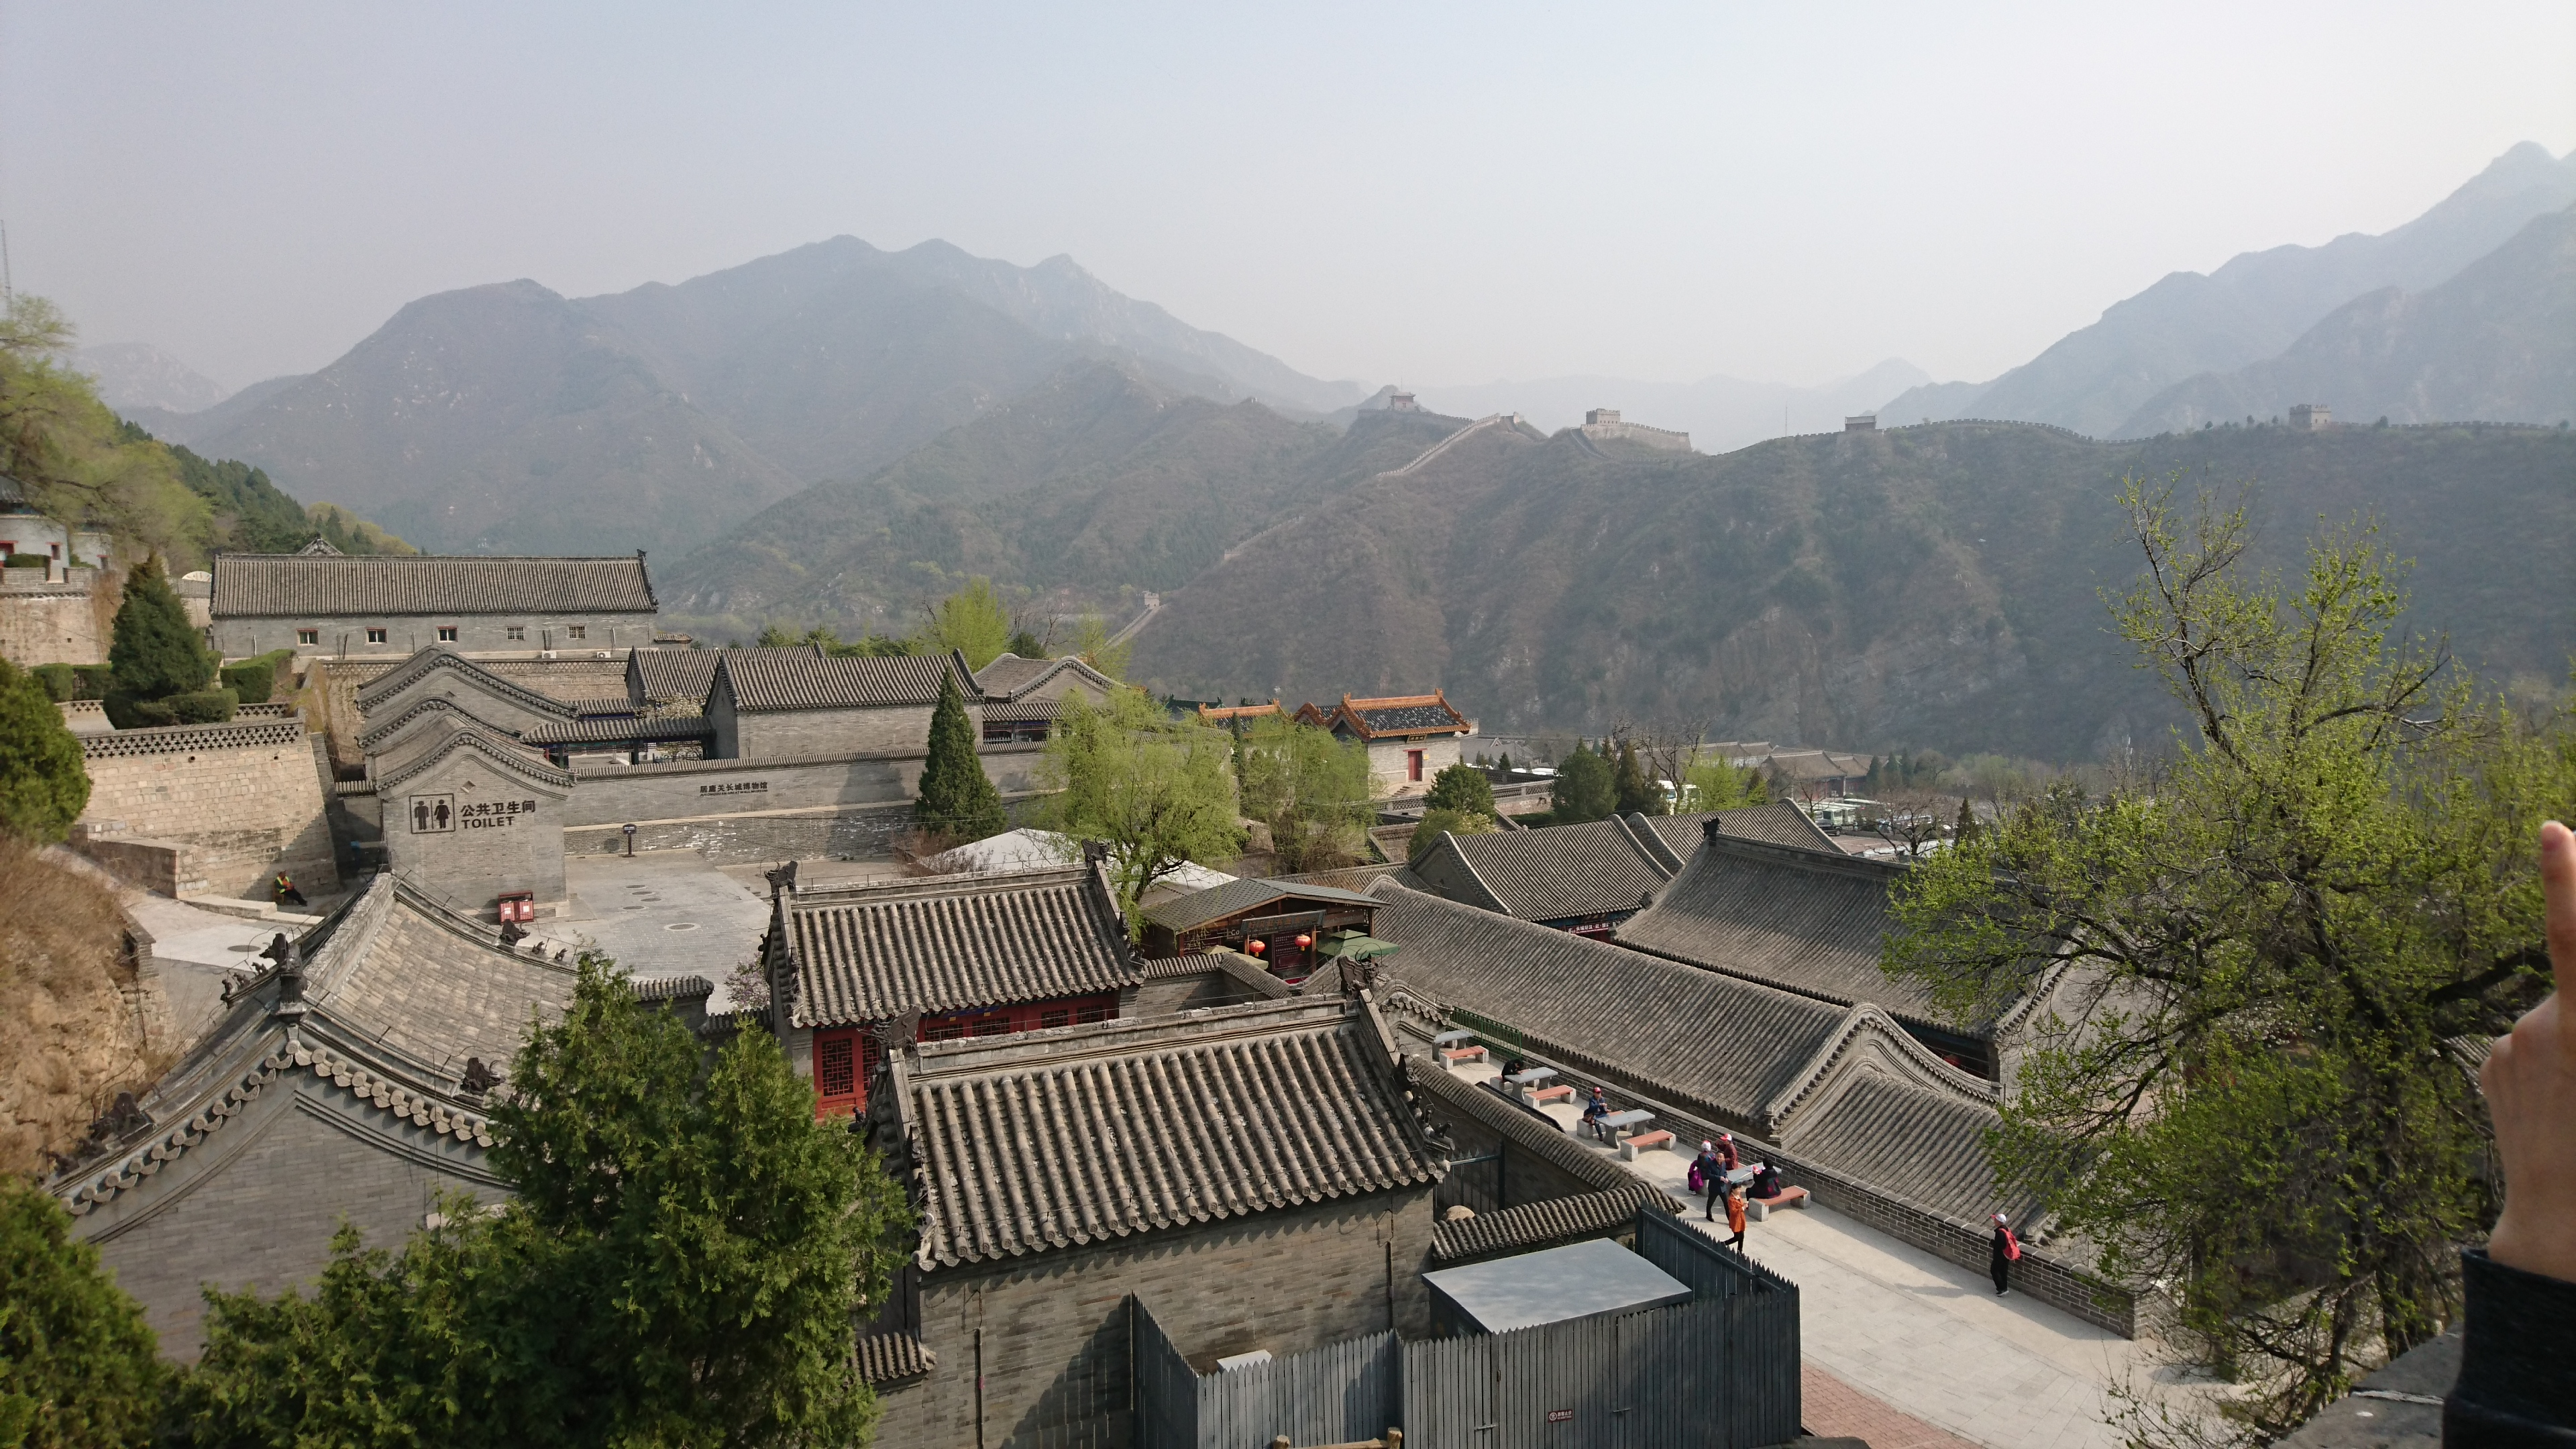
\includegraphics[width=1\textwidth]{icpc/DSC_0171}
  \column{0.5\textwidth}
  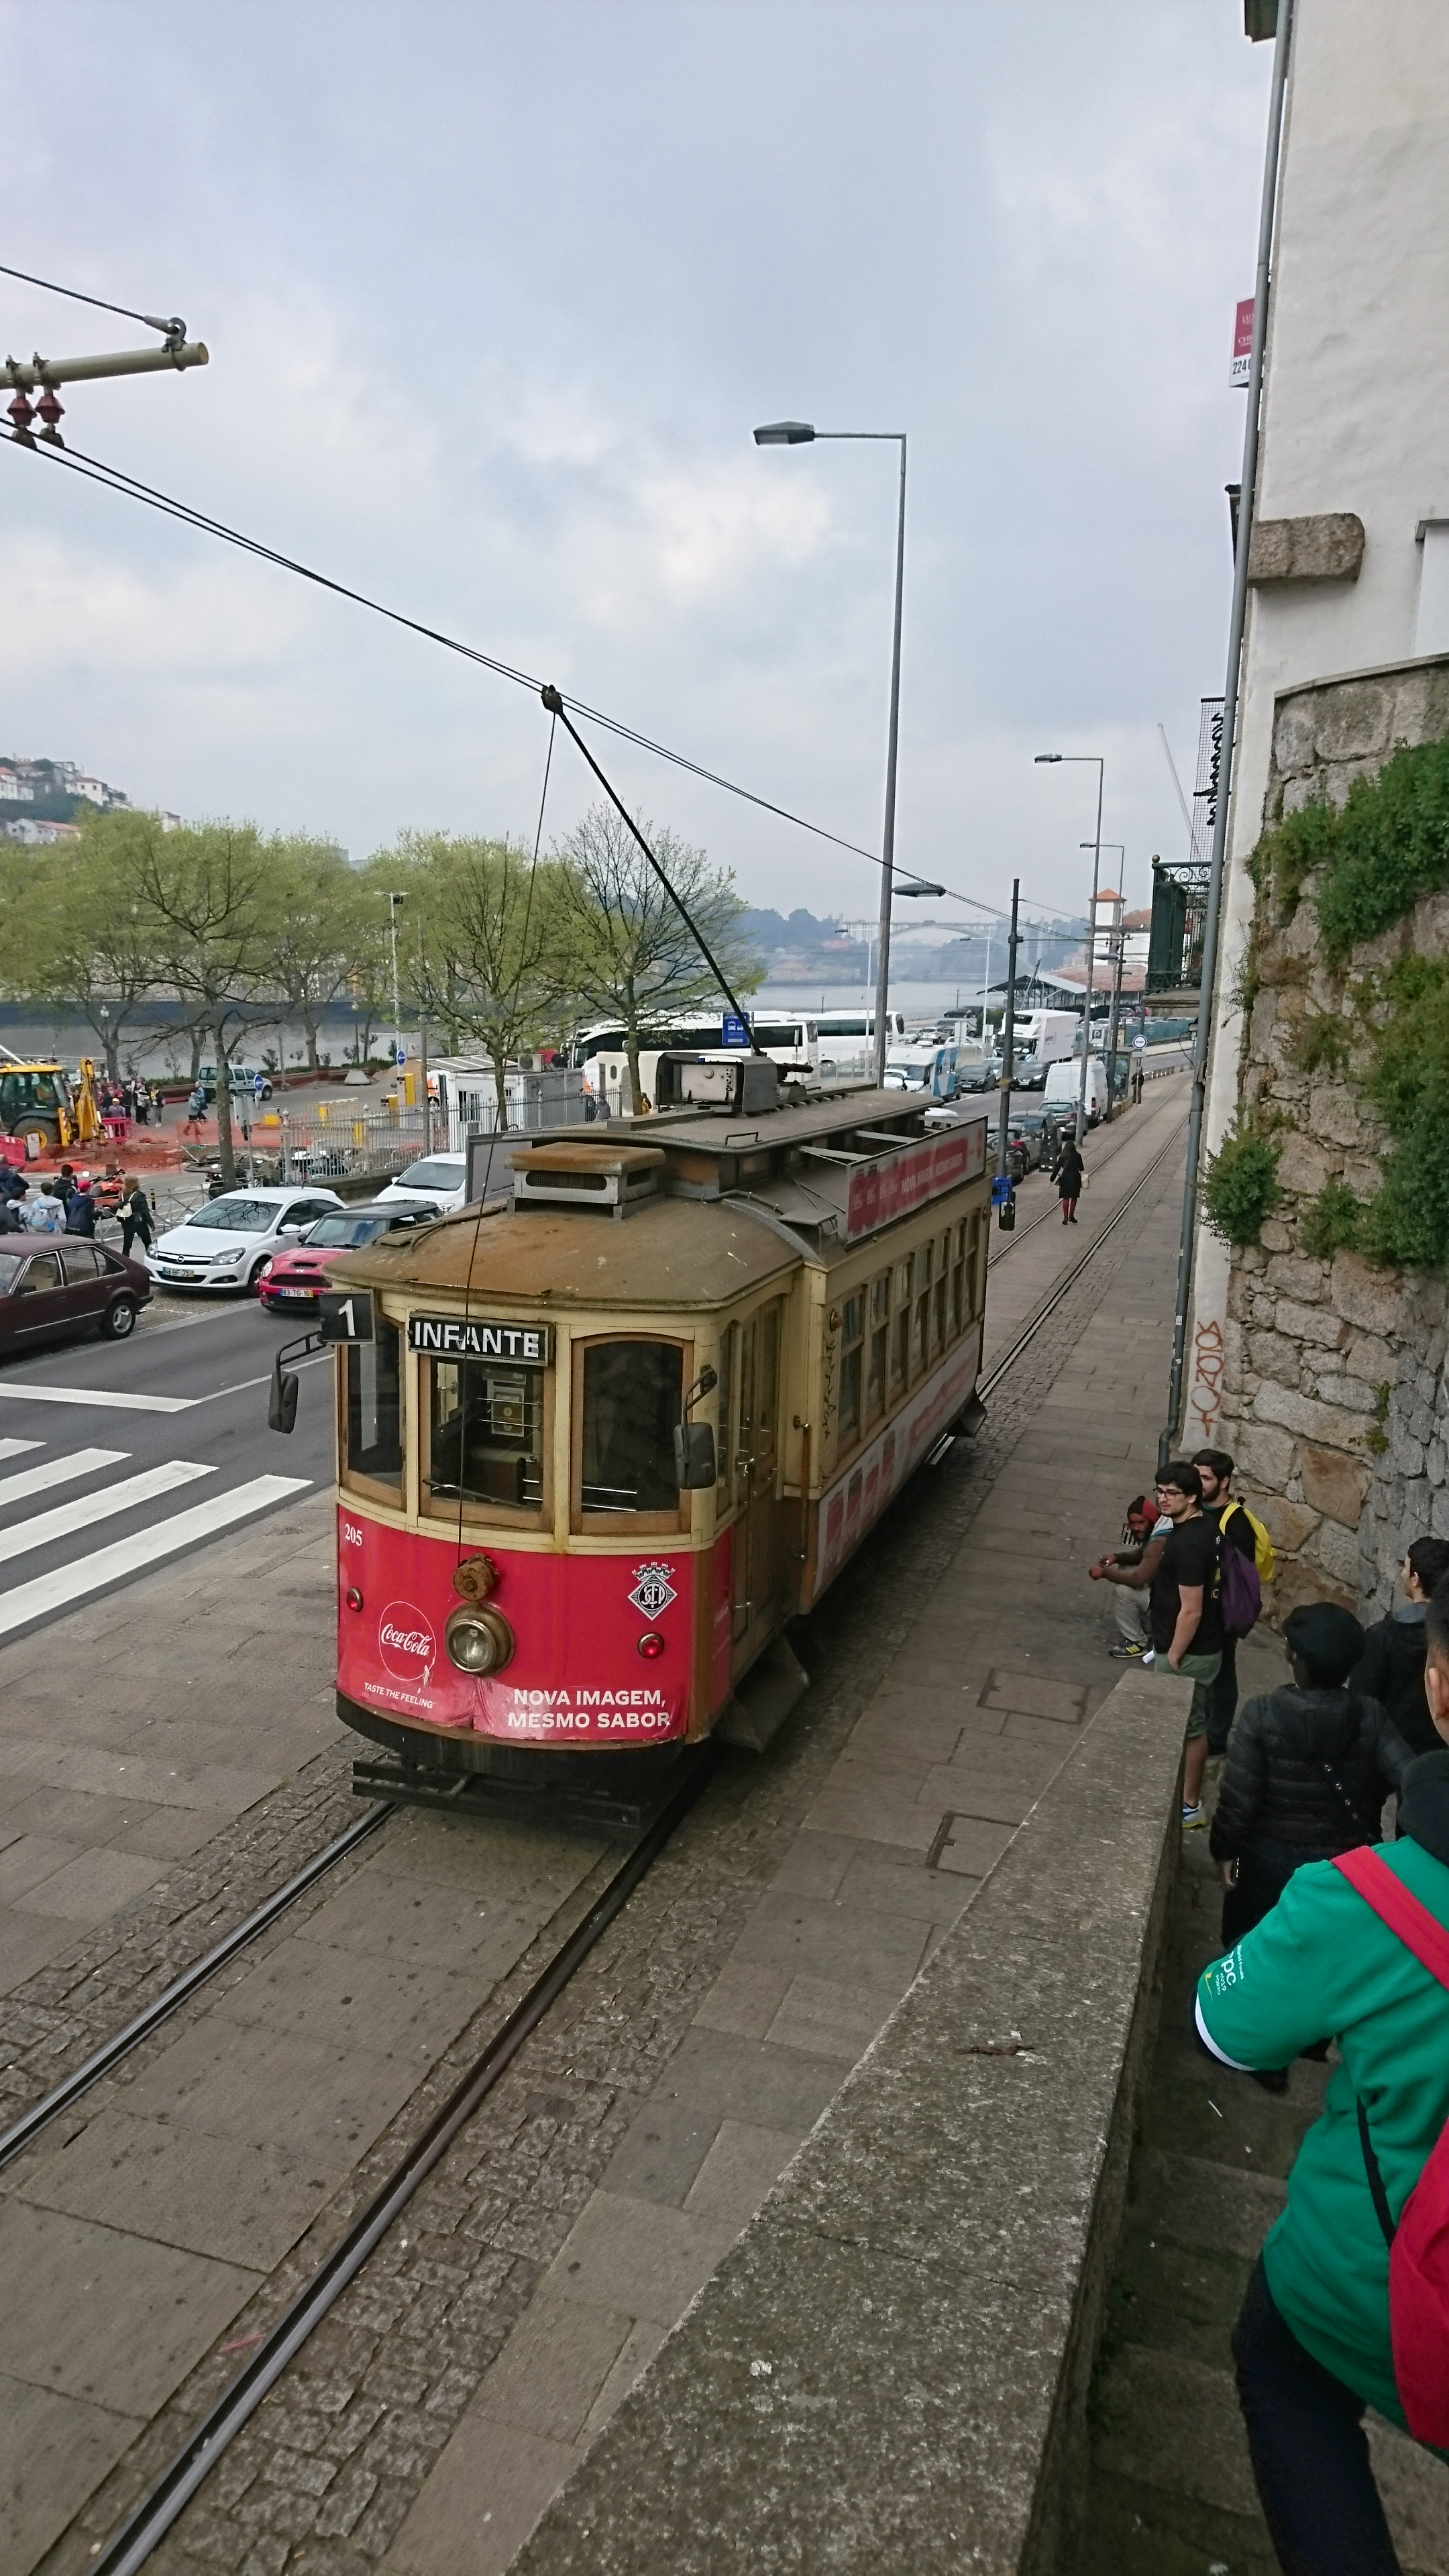
\includegraphics[width=1\textwidth]{icpc/DSC_0677}
\end{columns}


\end{frame}


\end{document}
